% Source: graduate-coursework/Sp26/CSCE775/Project/proposal_asv_3/proposal3_asv.tex
% Description: Network architecture. The policy network maps the 87D state through three hidden layers to a discrete mode head (4-way Gumbel-Softmax) and a continuous parameter head (7D with tanh activation). Twin critic networks (approximately 300k parameters each) take state-action pairs and output scalar $Q$-values.

\documentclass[border=4pt]{standalone}
\usepackage{amsmath,amssymb}
\usepackage{pgfplots}
\usepackage{tikz}
\usepackage{xcolor}
\pgfplotsset{compat=1.18}
\usetikzlibrary{positioning, arrows.meta, shapes.geometric, fit, calc, backgrounds, patterns, decorations.pathreplacing}

\definecolor{Garnet}{HTML}{73000A}
\definecolor{Atlantic}{HTML}{466A9F}
\definecolor{Congaree}{HTML}{1F414D}
\definecolor{Horseshoe}{HTML}{65780B}
\definecolor{Rose}{HTML}{CC2E40}
\definecolor{Honeycomb}{HTML}{A49137}
\definecolor{Black90}{HTML}{363636}
\definecolor{Black70}{HTML}{5C5C5C}
\definecolor{Black50}{HTML}{A2A2A2}
\definecolor{Black30}{HTML}{C7C7C7}
\definecolor{Black10}{HTML}{ECECEC}
\definecolor{WarmGrey}{HTML}{676156}


\begin{document}
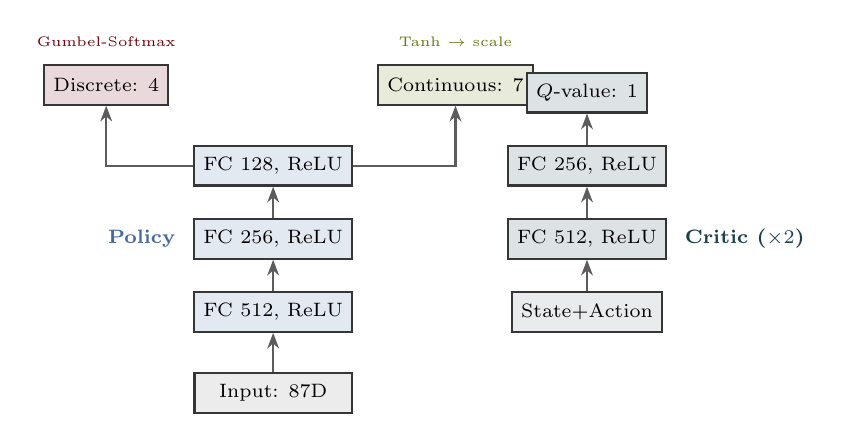
\begin{tikzpicture}[
    layer/.style={draw=Black90, thick, minimum width=1.6cm, minimum height=0.5cm, align=center, font=\scriptsize},
    head/.style={draw=Black90, thick, minimum width=1.4cm, minimum height=0.5cm, align=center, font=\scriptsize},
    arr/.style={-{Stealth[length=2mm]}, thick, color=Black70},
    every node/.style={font=\scriptsize}
]

% Policy Network
\node[layer, fill=Black10, minimum width=2.0cm] (input) {Input: 87D};
\node[layer, fill=Atlantic!15, above=0.5cm of input] (h1) {FC 512, ReLU};
\node[layer, fill=Atlantic!15, above=0.4cm of h1] (h2) {FC 256, ReLU};
\node[layer, fill=Atlantic!15, above=0.4cm of h2] (h3) {FC 128, ReLU};

% Discrete head
\node[head, fill=Garnet!15, above left=0.5cm and 0.3cm of h3] (disc) {Discrete: 4};
\node[font=\tiny, above=0.1cm of disc, color=Garnet] {Gumbel-Softmax};

% Continuous head
\node[head, fill=Horseshoe!15, above right=0.5cm and 0.3cm of h3] (cont) {Continuous: 7};
\node[font=\tiny, above=0.1cm of cont, color=Horseshoe] {Tanh $\rightarrow$ scale};

% Critic (side)
\node[layer, fill=Congaree!10, right=2.0cm of h1, minimum width=1.8cm] (ci) {State+Action};
\node[layer, fill=Congaree!15, above=0.4cm of ci] (ch1) {FC 512, ReLU};
\node[layer, fill=Congaree!15, above=0.4cm of ch1] (ch2) {FC 256, ReLU};
\node[head, fill=Congaree!15, above=0.4cm of ch2] (q) {$Q$-value: 1};

\draw[arr] (input) -- (h1);
\draw[arr] (h1) -- (h2);
\draw[arr] (h2) -- (h3);
\draw[arr] (h3) -| (disc);
\draw[arr] (h3) -| (cont);
\draw[arr] (ci) -- (ch1);
\draw[arr] (ch1) -- (ch2);
\draw[arr] (ch2) -- (q);

% Labels
\node[font=\scriptsize\bfseries, color=Atlantic, left=0.1cm of h2] {Policy};
\node[font=\scriptsize\bfseries, color=Congaree, right=0.1cm of ch1] {Critic ($\times 2$)};

\end{tikzpicture}
\end{document}
